% pruning.tex

\documentclass{standalone}
% newcommands.tex

\newcommand{\enq}{\texttt{enq}}
\newcommand{\deq}{\texttt{deq}}
\newcommand{\pput}{\texttt{PUT}}
\newcommand{\get}{\texttt{GET}}
\newcommand{\vs}{\texttt{vis}}
\newcommand{\so}{\texttt{so}}
\newcommand{\arb}{\texttt{ar}}
\newcommand{\rf}{\texttt{rf}}

% example
\newcommand{\po}[2]{\draw [->, thick] (#1) to node[above] {\Large{\so}} (#2);}
\newcommand{\pva}[2]{\draw [->, thick] (#1) to node[above] {$\Large{\so},\Large{\vs},\Large{\arb}$} (#2);}
\newcommand{\pbva}[2]{\draw [->, thick] (#1) to node[above] {$\Large{\so}$} node[below] {$\Large{\vs},\Large{\arb}$} (#2);}
\newcommand{\pv}[2]{\draw [->, thick] (#1) to node[above] {\Large{\so}} node[below] {\Large{\vs}} (#2);}
\newcommand{\evis}[2]{\draw [->, thick] (#1) to node[above, sloped, near end] {\Large{\vs}} (#2);}
\newcommand{\mvis}[2]{\draw [->, thick] (#1) to node[above, sloped] {\Large{\vs}} (#2);}
\newcommand{\ar}[2]{\draw [->, thick, allow upside down] (#1) to node[above, sloped] {\Large{\arb}} (#2);}
\newcommand{\va}[2]{\draw [->, thick, allow upside down] (#1) to node[above, sloped] {$\Large{\vs},\Large{\arb}$} (#2);}
\newcommand{\vab}[2]{\draw [->, thick, allow upside down] (#1) to node[below, sloped, near end] {$\Large{\vs},\Large{\arb}$} (#2);}
\newcommand{\vae}[2]{\draw [->, thick, allow upside down] (#1) to node[above, sloped, near end] {$\Large{\vs},\Large{\arb}$} (#2);}
\newcommand{\vas}[2]{\draw [->, thick, allow upside down] (#1) to node[sloped, near start, above] {$\Large{\vs},\Large{\arb}$} (#2);}

% serialization
\newcommand{\scc}[2]{\draw [->, very thick] (#1) to (#2);}
\newcommand{\rva}[2]{\draw [->, thick, allow upside down] (#1) to node[above, sloped] {$\Large{\rf},\Large{\vs},\Large{\arb}$} (#2);}
\newcommand{\rvb}[2]{\draw [->, thick, allow upside down] (#1) to node[below, sloped] {$\Large{\rf},\Large{\vs},\Large{\arb}$} (#2);}


\renewcommand{\keyxvar}{\textcolor{cyan}{\mathit{x}}}
\renewcommand{\keyyvar}{\textcolor{brown}{\mathit{y}}}

\usepackage{tikz}
\usetikzlibrary{shapes, positioning, arrows.meta, decorations.pathmorphing}

\begin{document}
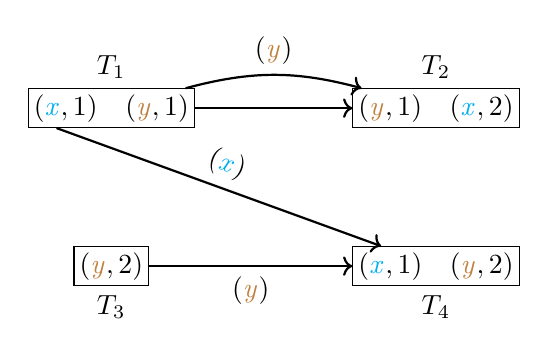
\begin{tikzpicture}[
  node distance = 1.5cm and 2.0cm,
  so/.style = {->, thick},
  wr/.style = {->, thick},
  ww/.style = {->, thick, dashed},
  rw/.style = {->, thick, dotted},
  txn/.style = {draw, inner sep = 2pt}]

  \node[txn, label = above : $T_{1}$] (t1) {$\writeevent(\keyxvar, 1) \quad \writeevent(\keyyvar, 1)$};
  \node[txn, label = above : $T_{2}$, right = of t1] (t2) {$\readevent(\keyyvar, 1) \quad \writeevent(\keyxvar, 2)$};

  \node[txn, below = of t1, label = below: $T_{3}$] (t3) {$\writeevent(\keyyvar, 2)$};
  \node[txn, below = of t2, label = below : $T_{4}$] (t4) {$\readevent(\keyxvar, 1) \quad \readevent(\keyyvar, 2)$};

  % t1 WR(y) t2
  \draw[wr, bend left = 15] (t1) to node[above]{$\WR(\keyyvar)$} (t2);
  % t1 SO t2
  \draw[so] (t1) to node[above]{$\SO$} (t2);
  % t3 WR(y) t4
  \draw[wr] (t3) to node[below]{$\WR(\keyyvar)$} (t4);
  % t1 WR(x) t4
  \draw[wr] (t1.200) to node[sloped, above]{$\WR(\keyxvar)$} (t4);
\end{tikzpicture}
\end{document}